This section describes the internal design of the elements of the
platform.
The GlobalController, the LocalControllers, and the Routers are shown
in more detail.

\subsection{The Global Controller}

The Global Controller is the main control point for the whole of VLSP.
It provides the Virtual Infrastructure Management (VIM) and
Orchestration Layer required to setup and manage virtual infrastructures.

\begin{figure}[h!]
    \centering
    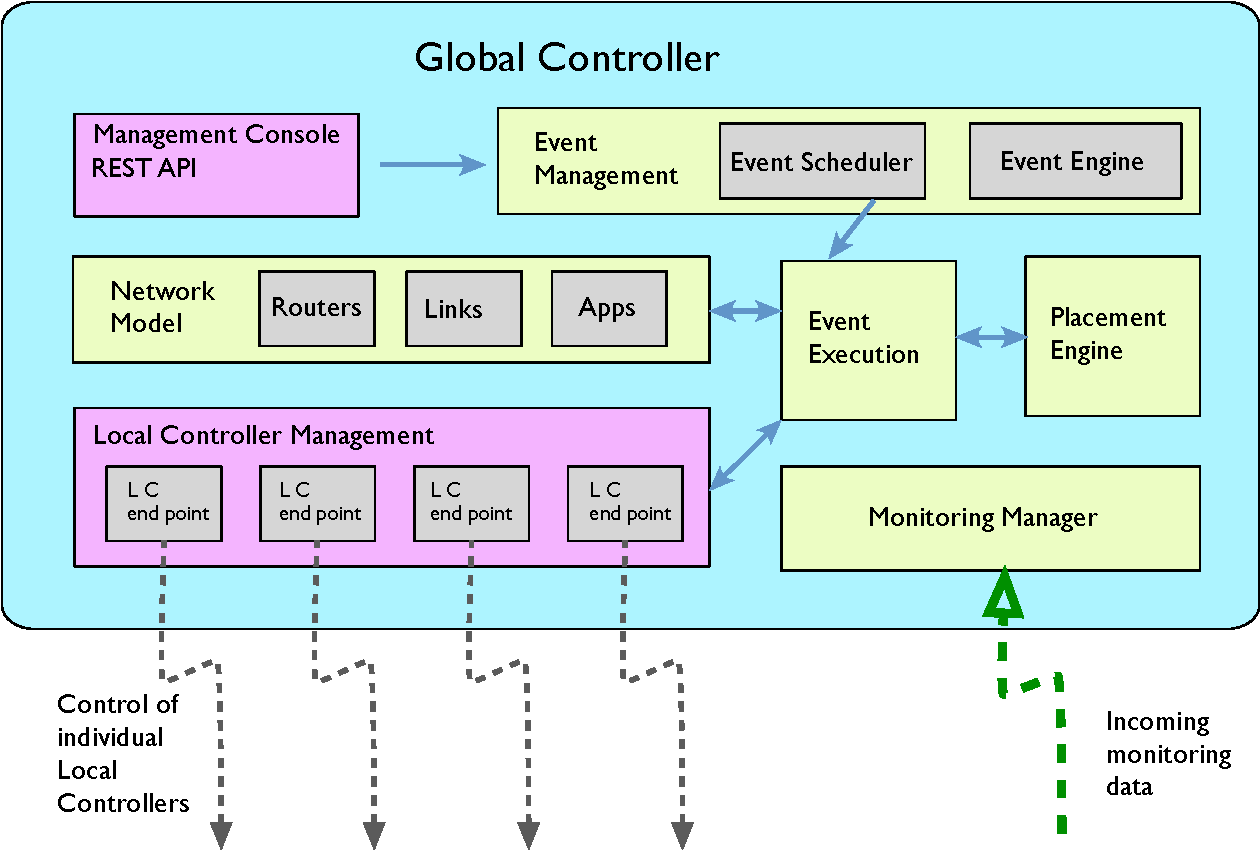
\includegraphics[width=14.5cm]{images/global_controller}
    \caption{Global Controller Architecture}
    \label{global-controller}
\end{figure}

The main elements of the Global Controller are:

\begin{description}[leftmargin=1.5em,labelindent=0,itemsep=3pt]

\item \textit{Event Management:} This is responsible for the runtime operation,
including support for event-based notifications and time scheduling of
events.  All setups that use the Probabilistic Experiment Control will
use an $Event Engine$ that generates events for router creation, link
creation, and router deletion.  These events are queued for
future activation in an $Event Scheduler$.  The configuration files
specify which probability distributions are used for these operations.

For setups using the REST API for Dynamic Programmable Control, the
call to the Management Console is converted into an event that
executes immediately.

\item \textit{Management Console - REST API:} This is an HTTP listener
  that supports the REST API into the Global Controller, and essentially the whole
  of VLSP.

\item \textit{Event Execution:} This executes the actions for each of
the events that the  $Event Scheduler$ chooses as the next action.
Each Event has a time, an event type, and some event
parameters. During event execution there is a handler for each type of
event, which causes the relevant actions to be performed.

\item \textit{Placement Engine:} This decides where to place a new
  router when one is created. The Placement Engine uses data about the
  current state, context, and configuration of the system to choose a
  location. The Placement Engine is a flexible part of VLSP and can be
  changed at run-time under software control.

\item \textit{Network Model:} This keeps information on the topology
  of the virtual network that has been created and is being managed,
  including all of the $Routers$ and $Links$. It also contains
  information on the $Apps$ that are running on eahc virtual router.
  The Model is used by many components in the Global Controller for
  decision making, outputs via the REST API, as well as visualization.

\item \textit{Monitoring Manager:} This manages the monitoring
  sub-system of VLSP.  It starts any configured probes on the virtual
  routers, and starts any configured data consumers and data reporters. The monitoring
  data is used by many components inside the Global Controller.

\item \textit{Local Controller Management:}  This is responsible for
  starting Local Controllers on specified hosts, interacting directly
  with those Local Controllers, and managing their state.  This
  element has an $end-point$ for each Local Controller that has been
  defined, as well as a direct network connection to that Local
  Controller for sendign it commands.

  All operations to start and stop routers, and commands for routers
  are directed through the relevant Local Controller.

  
\end{description}


\subsubsection{Management Console}

The Management Console supports the REST API into the Global
Controller.
All of the REST commands are presented in Appendix \ref{chap:restapi}.

\subsubsection{Placement Engine}

We have experimented with various placement algorithms, more details
of which can be found in our other papers. The \emph{Placement
Engine} of VLSP is the management component in charge of performing the
actual placement of the virtual entities and the application nodes
they host, according to the initial topology and the resource usage of
the virtual network elements. This is an important feature because,
when we configure a network or a service, given initial context
information, some of these parameters may change during the course of
the system’s operation and a reconfiguration may be required to
maintain optimized behaviour. Consequently, our approach has a
mechanism to achieve adaptation in a flexible manner.

The decision of the \emph{Placement Engine}, which can be changed at
run-time under software control, is encoded in an algorithm which can
be either rather simple, such as counting the number of virtual
routers on a host, or it can be complex, based on a set of constraints
and policies that represent the network properties. Therefore, to
determine the placement for the ‘next’ virtual router, the
GlobalController uses the defined Placement Engine.

The name of the Placement Engine class is set in the
\texttt{<PlacementEngineClass>} field.
The default class name is: \texttt{usr.globalcontroller.LeastUsedLoadBalancer}.
This is a list of the current implementations:

\begin{adjustwidth}{\parindent}{} % was 2em but \parindent is better
\begin{verbatim}
usr.globalcontroller.LeastBusyPlacement
usr.globalcontroller.LeastUsedLoadBalancer
usr.globalcontroller.NupPlacement
usr.globalcontroller.EnergyEfficientPlacement
\end{verbatim}
\end{adjustwidth}


\noindent The user can write their own Placement Engine, and set it in the
config  Such a Placement Engine can take into account any attributes
that are needed to make a decision 
which chooses a particular Local Controller.

\subsubsection{Monitoring Manager}

The Monitoring Manager is responsible for starting, stopping, and
processing the monitoring processes within VLSP.
Probes can be configured to start in the Routers which send various
kinds of measurment data related to different router processes and
tasks.

\subsubsection*{Router Probes}

The current set of probes that have been defined are:


{
  \small

  \begin{longtable}{ | p{5.7cm} | p{8.7cm} | }

\hline
\textbf{Name} & \textbf{Description} \\
\hline
\texttt{usr.router.AppListProbe} & This probe sends a list of all the executing
applications in a router. \newline
% /tmp/gc-channel10.out
The probe sends the \texttt{RouterName} plus
a table of \texttt{Data} with 1 row per app.

\vspace{\baselineskip}
\begin{tabular}{ p{8.3cm} }
  \hline
  ProbeAttributeType.STRING \\
  \hline
  \texttt{RouterName} \\
  \hline
  TableProbeAttribute \\
  \hline
  \texttt{Data} \\
  \hline 
\begin{lstlisting}[language=java] 
"AID", ProbeAttributeType.INTEGER
"StartTime", ProbeAttributeType.LONG
"ElapsedTime", ProbeAttributeType.LONG
"RunTime", ProbeAttributeType.LONG
"UserTime", ProbeAttributeType.LONG
"SysTime", ProbeAttributeType.LONG
"State", ProbeAttributeType.STRING
"ClassName", ProbeAttributeType.STRING
"Args", ProbeAttributeType.STRING
"Name", ProbeAttributeType.STRING
"RuntimeKeys", ProbeAttributeType.LIST
"RuntimeValues", ProbeAttributeType.LIST
\end{lstlisting} \\
  \hline
\end{tabular}

\\
\hline
\texttt{usr.router.NetIFStatsProbe} & This probe sends a list of stats
for each of the network interfaces of the Router. \newline
% /tmp/gc-channel7.out 
The probe sends the \texttt{RouterName} plus
a table of \texttt{Data} with 1 row per app.

\vspace{\baselineskip}
\begin{tabular}{ p{8.3cm} }
  \hline
  ProbeAttributeType.STRING \\
  \hline
  \texttt{RouterName} \\
  \hline
  TableProbeAttribute \\
  \hline
  \texttt{Data} \\
  \hline
\begin{lstlisting}[language=java]
"name", ProbeAttributeType.STRING
"InBytes", ProbeAttributeType.INTEGER
"InPackets", ProbeAttributeType.INTEGER
"InErrors", ProbeAttributeType.INTEGER
"InDropped", ProbeAttributeType.INTEGER
"InDataBytes", ProbeAttributeType.INTEGER
"InDataPackets", ProbeAttributeType.INTEGER
"OutBytes", ProbeAttributeType.INTEGER
"OutPackets", ProbeAttributeType.INTEGER
"OutErrors", ProbeAttributeType.INTEGER
"OutDropped", ProbeAttributeType.INTEGER
"OutDataBytes", ProbeAttributeType.INTEGER
"OutDataPackets", ProbeAttributeType.INTEGER
"InQueue", ProbeAttributeType.INTEGER
"BiggestInQueue", ProbeAttributeType.INTEGER
"OutQueue", ProbeAttributeType.INTEGER
"BiggestOutQueue", ProbeAttributeType.INTEGER
\end{lstlisting} \\
\hline
\end{tabular}

\\
\hline
\texttt{usr.router.ThreadGroupListProbe} & This probe sends data for
each Thread Group in the Router.  \newline
%/tmp/gc-channel14.out
The probe sends the \texttt{RouterName} plus
a table of \texttt{Data} with 1 row per app.

\vspace{\baselineskip}
\begin{tabular}{ p{8.3cm} }
  \hline
  ProbeAttributeType.STRING \\
  \hline
  \texttt{RouterName} \\
  \hline
  TableProbeAttribute \\
  \hline
  \texttt{Data} \\
  \hline
\begin{lstlisting}[language=java]
"Name", ProbeAttributeType.STRING
"StartTime", ProbeAttributeType.LONG
"ElapsedTime", ProbeAttributeType.LONG
"RunTime", ProbeAttributeType.LONG
"UserTime", ProbeAttributeType.LONG
"SysTime", ProbeAttributeType.LONG
"Mem", ProbeAttributeType.LONG
\end{lstlisting} \\
\hline
\end{tabular}

\\
\hline
\texttt{usr.router.ThreadListProbe} & This probe sends data for
each Thread Group in the Router.  \newline
% /tmp/gc-channel15.out
The probe sends the \texttt{RouterName} plus
a table of \texttt{Data} with 1 row per app.


\vspace{\baselineskip}
\begin{tabular}{ p{8.3cm} }
  \hline
  ProbeAttributeType.STRING \\
  \hline
  \texttt{RouterName} \\
  \hline
  TableProbeAttribute \\
  \hline
  \texttt{Data} \\
  \hline
\begin{lstlisting}[language=java]
"Name", ProbeAttributeType.STRING
"StartTime", ProbeAttributeType.LONG
"ElapsedTime", ProbeAttributeType.LONG
"RunTime", ProbeAttributeType.LONG
"UserTime", ProbeAttributeType.LONG
"SysTime", ProbeAttributeType.LONG
"Mem", ProbeAttributeType.LONG
"ThreadGroup", ProbeAttributeType.STRING
\end{lstlisting} \\
\hline
\end{tabular}

\\
\hline
\end{longtable}


\normalsize
}


\subsubsection*{Local Controller Probe}

There is currently one probe residing in the Local Controller.
It is turned on automatically if monitoring is configured to be on.
This probe is designed to send host based info back to the Global
Controller. 


{
  \small

  \begin{longtable}{ | p{5.7cm} | p{8.7cm} | }

\hline
\textbf{Name} & \textbf{Description} \\
\hline
\texttt{usr.localcontroller. HostInfoProbe} & This probe sends data
about the physical host that the LocalController is managing. \newline
% /tmp/gc-channel13.out
The probe sends the \texttt{Name} of the host, cpu usage, memory usage,
plus a table of network statistics, with 1 row per network interface
of the physical host.

\vspace{\baselineskip}
\begin{tabular}{ p{8.3cm} }
  \hline
  ProbeAttributeType.STRING \\
  \hline
  \texttt{Name} \\
  \hline
  ProbeAttributeType.FLOAT \\
  \hline
  \texttt{cpu-user} \\
  \hline
  ProbeAttributeType.FLOAT \\
  \hline
  \texttt{cpu-sys} \\
  \hline
  ProbeAttributeType.FLOAT \\
  \hline
  \texttt{cpu-idle} \\
  \hline
  ProbeAttributeType.FLOAT \\
  \hline
  \texttt{load-average} \\
  \hline
  ProbeAttributeType.INTEGER \\
  \hline
  \texttt{mem-used} \\
  \hline
  ProbeAttributeType.INTEGER \\
  \hline
  \texttt{mem-free} \\
  \hline
  ProbeAttributeType.INTEGER \\
  \hline
  \texttt{mem-total} \\
  \hline
  TableProbeAttribute \\
  \hline
  \texttt{net-stats} \\
  \hline
\begin{lstlisting}[language=java]
"if-name", ProbeAttributeType.STRING
"in-packets", ProbeAttributeType.LONG
"in-bytes", ProbeAttributeType.LONG
"out-packets", ProbeAttributeType.LONG
"out-bytes", ProbeAttributeType.LONG
\end{lstlisting} \\
  \hline
\end{tabular}

\\
\hline
  \end{longtable}

 
\normalsize
}

\subsubsection*{Global Controller Reporters}

The reporters which can be configured in the Global Controller are
designed to collect measurements which are sent by the probes in other
parts of the system.


The current set of probes that have been defined are:


{
  \small

  \begin{longtable}{ | p{5.7cm} | p{8.7cm} | }

\hline
\textbf{Name} & \textbf{Description} \\
\hline
\texttt{usr.globalcontroller. HostInfoReporter} & This reporter
collects measurements from the \texttt{HostInfoProbe} embedded in the
Local Controller.

Additionally data is sent to /tmp/gc-channel13.out.
\hline
\texttt{usr.globalcontroller. RouterAppsReporter} & This reporter
collects measurements from the \texttt{AppListProbe} embedded in the
router, if it has been configured.

Additionally data is sent to /tmp/gc-channel10.out.
\hline
\texttt{usr.globalcontroller. NetIFStatsReporter} & This reporter
collects measurements from the \texttt{NetIFStatsProbe} embedded in the
router, if it has been configured.

Additionally data is sent to /tmp/gc-channel7.out.
\hline
\texttt{usr.globalcontroller. ThreadGroupListReporter} & This reporter
collects measurements from the \texttt{ThreadGroupListProbe} embedded in the
router, if it has been configured.

Additionally data is sent to /tmp/gc-channel14.out.
\hline
\texttt{usr.globalcontroller. ThreadListReporter} & This reporter
collects measurements from the \texttt{ThreadListProbe} embedded in the
router, if it has been configured.

Additionally data is sent to /tmp/gc-channel15.out.
\hline
  \end{longtable}

 
\normalsize
}


\subsection{The Local Controller}

The Local Controller is a per host Host Controller that accepts
commands that are specifically for that host.
The Local Controller acts as a management point for starting and
stopping Routers, for creating and deleting links, and also for
monitoring the host it runs on.

\subsection{Routers}

The Routers themselves have multiple network interfaces, one interface
for each connection to another router, as well as 6 internal main
functional blocks.

\begin{figure}[h!]
    \centering
    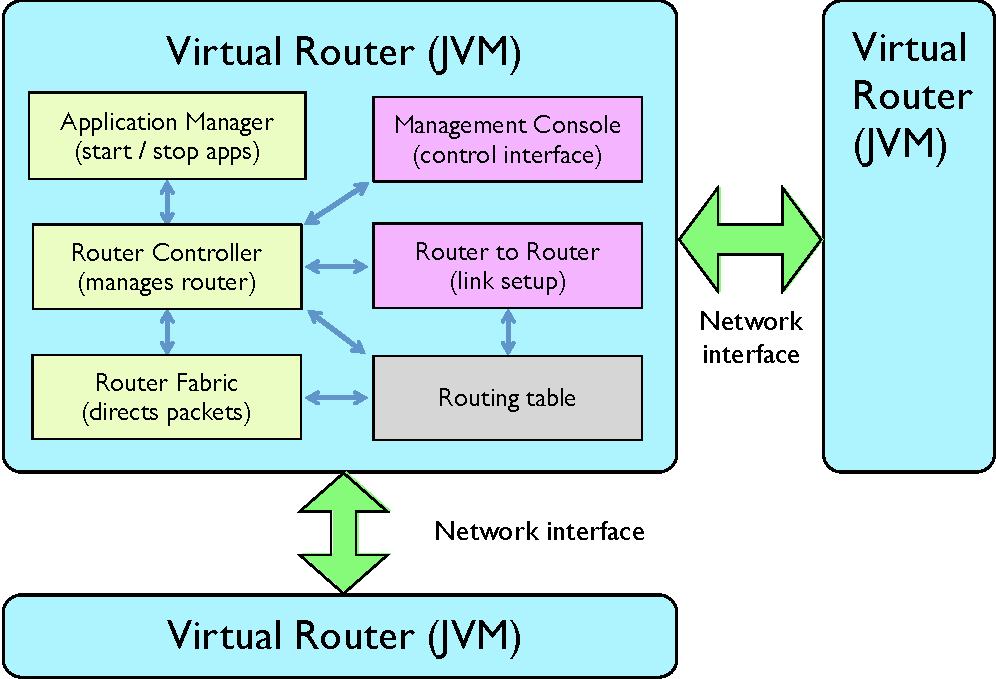
\includegraphics[width=11cm]{images/router-main-blocks}
    \caption{Router Top Level View with Main Functional Blocks}
    \label{design:router-main-blocks}
\end{figure}





The Router functions include:

\begin{itemize}

\item \emph{Management Console} -- which provides a control interface from the
  outside world

\item \emph{Router to Router} -- which provides the mechanism to setup new
  connections to other routers

\item \emph{Router Controller} -- which controls the internal operation of
  the router

\item \emph{Router Fabric} -- which connects the network interfaces to
  the router and provides the forwarding mechanism

\item \emph{Routing Table} -- which holds information about how to
  route datagrams

\item \emph{Application Manager} -- which starts up and shuts down
  applications that might run on the router

\end{itemize}

\noindent Each of these is shown in figure \ref{design:router-main-blocks}.



Each of the functional blocks is manifested into an design
element within the interal architecture of the router.


\begin{figure}[h!]
    \centering
    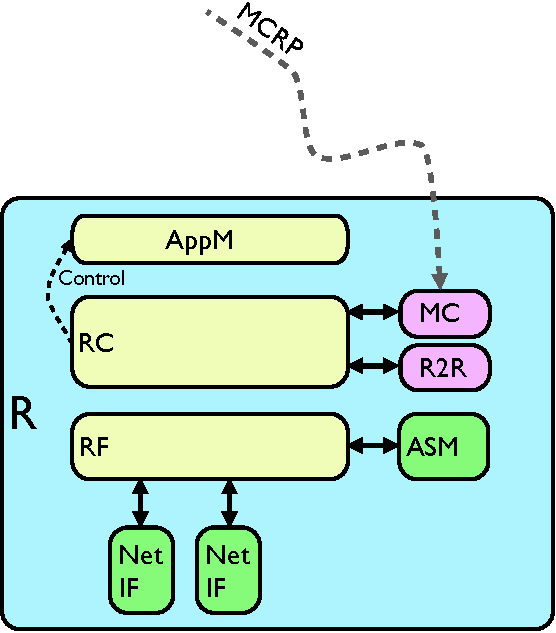
\includegraphics[width=7cm]{images/router-elements}
    \caption{Router Internal Architecture}
    \label{design:router-elements}
\end{figure}


These functions include:

\begin{itemize}

\item \emph{MC} -- Management Consolewhich provides a control interface from the
  outside world

\item \emph{R2R} -- Router to Router which provides the mechanism to setup new
  connections to other routers

\item \emph{RC} -- Router Controller which controls the internal operation of
  the router

\item \emph{RF} -- Router Fabric which connects the network interfaces to
  the router and provides the forwarding mechanism

\item \emph{AppM} -- Application Manager which starts up and shuts down
  applications that might run on the router

\item \emph{NetIF} -- a Network Interface to another virtual Router.

\item \emph{ASM} -- the Application Socket Mux - which is the Network
  Interface to the local router. All \emph{Sockets} for local apps are
  multiplexed through this interface.

\end{itemize}

\noindent Each of these is shown in figure \ref{design:router-elements}.



\subsubsection{Connecting Routers}

In this section the mechanism by whch one Router connects to another
Router in order to create a new virtual network connection is shown.

Each virtual router is connected directly to another virtual router
via a Network Interface (NetIF).
The connection can be configured to be a TCP connection or a UDP
connection.

The TCP connection gives an underlying transport for the traffic that
is reliable. 

The UDP connection gives an underlying transport for the traffic that
is unreliable.

In figure \ref{design:two-routers}, two apps are started on a Router,
each with it's own Socket.  We see how the Socket is connected to the
Router Fabric via the ASM.

\begin{figure}[h!]
    \centering
    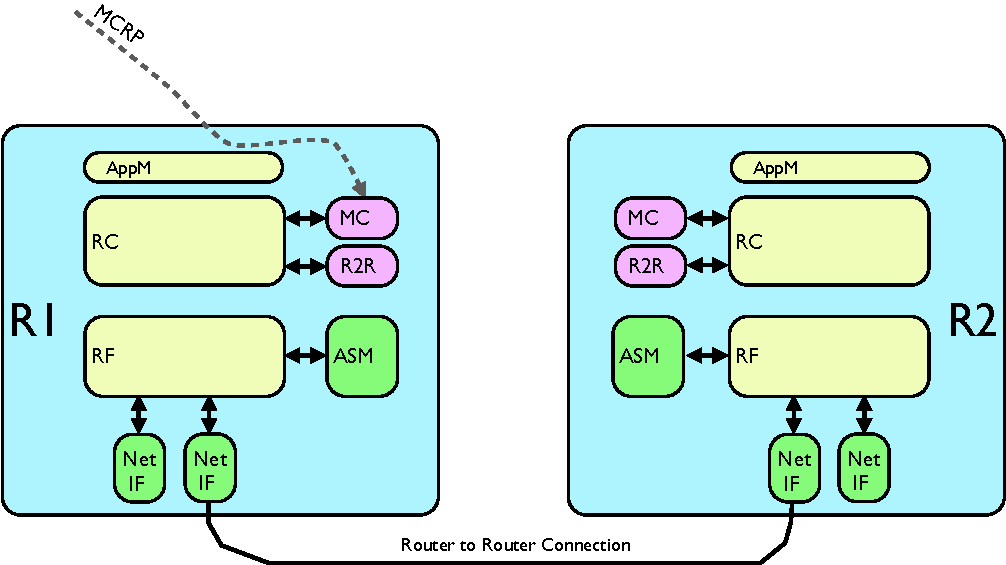
\includegraphics[width=12cm]{images/two-routers}
    \caption{Two Routers}
    \label{design:two-routers}
\end{figure}

\subsubsection{Applications and Application Lifecycle}

Applications and services on the platform are run as applications on a router.

Each router has a local network interface that provides a Socket level
API for these applications.  In appendix \ref{chap:methods}, there is
are full details of this API.

This Socket level API presents a UDP-like socket that can be used for
writing networking applications that run directly on the router.
These applications are started at run-time by making a call to the
Global Controller, passing in the name of the class and the arguments
it needs to start up.


\begin{figure}[h!]
    \centering
    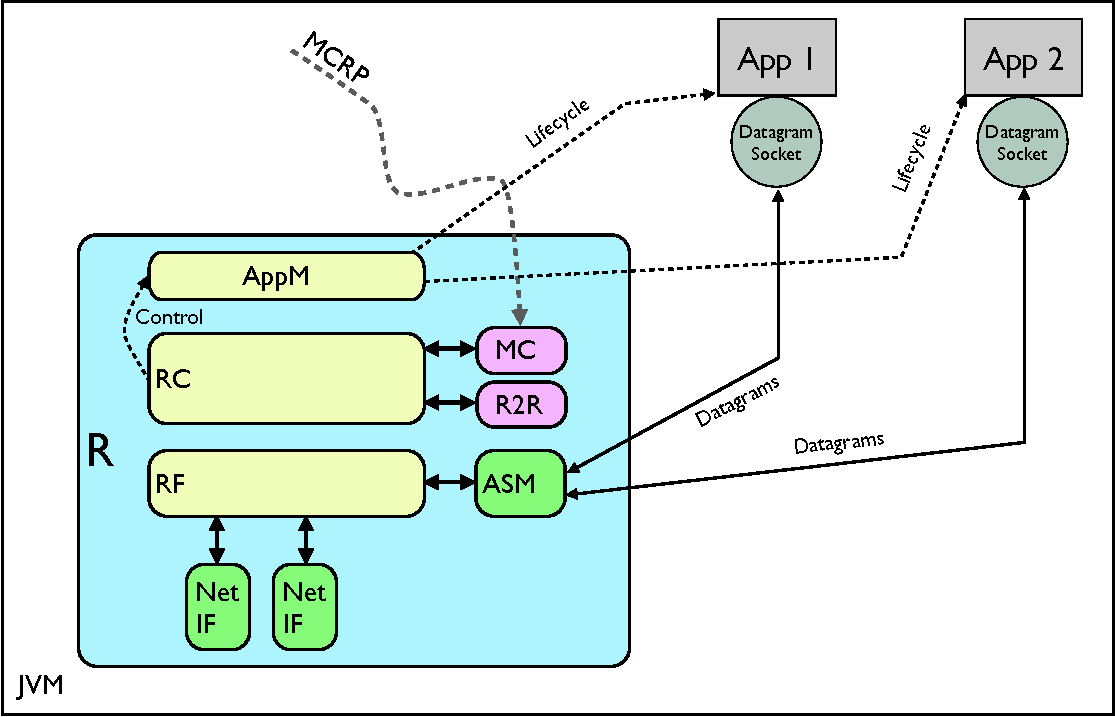
\includegraphics[width=11cm]{images/app-manager}
    \caption{Application Manager and Application Lifecycle}
    \label{design:app-manager}
\end{figure}



